\documentclass[11pt]{article}
\usepackage[letterpaper,margin=0.9in]{geometry}
\usepackage{amsmath,amssymb,amsthm,graphicx}
\usepackage[hidelinks]{hyperref}
\newtheorem*{theorem}{Theorem}
\newcommand{\Rea}{\operatorname{Re}}
\title{A quantum clock for the cubic of discriminant 229\\
\large Finite Weil positivity and a test on perfect powers}
\author{}\date{}
\begin{document}
\maketitle
\vspace{-2.6em}
Let $F=\mathbb Q[x]/(x^3-4x-1)$ and write $A=\zeta_F/\zeta$ for its standard
two-dimensional Artin factor. Two adjacent intervals of length $L$, with weights
$+1$ and $-1$, define a Haar function. Its Weil quadratic form $H(L)$ is
computable from prime powers through $X=e^{2L}$. An off-line zero forces
both signs of large excursions of $H$, even at cutoffs $X=n^{100}$.
We also construct a finite unitary clock from the prime side. Its correlations
realize the Weil form for all superpositions of 160 consecutive cells.
The finite certificate uses no zero ordinates.

\section*{1. The observable}
For $\Phi_L(u)=(L-|u|)_+$, put $V(L)=W_A(\Phi_L)$ and
$H(L)=4V(L)-V(2L)$. Indeed $4\Phi_L-\Phi_{2L}$ is the autocorrelation
of $\mathbf1_{[0,L]}-\mathbf1_{[L,2L]}$. Use the Fourier convention
$\widehat\Phi(t)=\int\Phi(u)e^{itu}\,du$. At a good prime put
$b(p^j)=\#\{x\in\mathbb F_{p^j}:x^3-4x-1=0\}-1$.
The reciprocal Euler polynomial at the ramified prime is $1-p^{-s}$,
so $b(229^j)=1$. The prime-side formula is
\begin{align}
 V(L)&=D(L)-2\sum_{q=p^j}\frac{b(q)\log p}{\sqrt q}(L-\log q)_+,\label{eq:prime}\\
 D(L)&=cL+4\sum_{m\ge0}\frac{1-e^{-(2m+1/2)L}}{(2m+1/2)^2},\qquad
 c=\log(229/\pi^2)-2\gamma-\pi-6\log2. \label{eq:arch}
\end{align}
Both gamma factors are $\Gamma_{\mathbb R}(s)=\pi^{-s/2}\Gamma(s/2)$.
Subtract $\psi(1/4)$ from $\Rea\psi(1/4+it/2)$ in the explicit formula.
The digamma integral and Fourier inversion give the remainder
\[
 4\int_0^\infty \frac{e^{-u/2}\min(u,L)}{1-e^{-2u}}\,du.
\]
Integrating term by term gives \eqref{eq:arch}. The constant follows from
$2\psi(1/4)=-2\gamma-\pi-6\log 2$.

Write $z=\rho-1/2$ for the centered nontrivial zeros of $A$, counted with
multiplicity. The zero side of the explicit formula gives
\[
 V(L)=\sum_z\frac{e^{zL}+e^{-zL}-2}{z^2}.
\]
At $z=0$ the summand is $L^2$. Under GRH the central contribution cancels and
\[
 H(L)=\sum_{\gamma\ne0}\frac{4(1-\cos L\gamma)^2}{\gamma^2}
 \qquad(\rho=1/2+i\gamma).
\]
Thus $H$ is bounded and nonnegative under GRH. The triangle function is
closely related to Suzuki's screw function \cite{suzuki,form}. The block
correlations below are finite differences of this function.

\newpage
\section*{2. Sampling on arbitrarily high perfect powers}
Write $u_+=\max(u,0)$ and $\Theta=\sup_\rho(\Rea\rho-1/2)$. The functional
equation gives $0\le\Theta\le1/2$.
\begin{theorem}
Fix any $K>0$ and put $L_n=(K/2)\log n$. For each sign separately,
\[
 \boxed{\displaystyle
 \limsup_{n\to\infty}
 \frac{\log(1+(\pm H(L_n))_+)}{\log(n^K)}=\Theta .}
\]
In particular, a lower bound $H(L_n)\ge-C_\varepsilon(n^K)^\varepsilon$
for every $\varepsilon>0$ and all sufficiently large $n$ implies GRH for $A$.
\end{theorem}
\begin{proof}
The zero expansion gives $|H(t)|\ll e^{2\Theta t}$ since the central
contribution cancels and $\sum_{z\ne0}|z|^{-2}<\infty$. If $\Theta=0$ this
proves the claim. Suppose $\Theta>0$. First consider the continuous limsup
for each sign with denominator $t$.

Let $B(s)=\int_0^\infty e^{-st}V(t)\,dt$, initially for $\Rea s>\Theta$.
The zero sum integrates to
\[
 B(s)=\sum_z\frac{2}{s(s^2-z^2)},\qquad
 \mathcal L H(s)=4B(s)-\tfrac12 B(s/2).
\]
The series is normally convergent locally away from $0$ and its poles.
At $s=z\ne0$ the terms from $z$ and $-z$ reinforce by the functional
equation. The bilateral Laplace kernel for the completed $A$ is strictly
positive by the companion cubic note \cite{cubic}. Thus $B$ has no pole
on the positive real axis. The transform of $H$ has poles at $s=2z$ with
real parts arbitrarily close to $2\Theta$. At $2\Rea z>\Theta$ the first
term is holomorphic there.

If either sign of $H$ had positive-part growth exponent less than $2\Theta$,
there would be $0<b<2\Theta$ and $C>0$ such that $Ce^{bt}+H(t)$ or
$Ce^{bt}-H(t)$ were nonnegative on $t\ge0$. Its Laplace transform has a
pole with real part $>b$, yet is holomorphic at every real $s>b$. This
contradicts Landau's theorem that the finite abscissa of convergence of a
nonnegative Laplace integral is a real singularity. The continuous limsup
for each sign is therefore $2\Theta$.

For $0\le h\le1$ we have
$|e^{\pm zh}-1|\ll\min(1,|z|h)\ll |z|^{1/2}h^{1/2}$.
The degree-two zero count $N(T)=O(T\log(2+T))$ gives
$\sum_{z\ne0}|z|^{-3/2}<\infty$. Applying the bound to both scales gives
\[
 |H(t+h)-H(t)|\ll e^{2\Theta t}h^{1/2}.
\]
Successive samples near $t$ are $O_K(e^{-2t/K})$ apart. Interpolation
costs $O_K(e^{(2\Theta-1/K)t})$, a strict saving in the exponent for
every fixed $K$. A smaller signed limsup at the samples would force a
smaller continuous limsup. Division by $\log(n^K)=2L_n$ finishes the proof.
\end{proof}
The proof also applies to self-dual entire completed $L$-functions with
the same zero-count bound, functional symmetry and no noncentral real zeros.
It gives an asymptotic detection result without a bound on the first failure.

\newpage
\section*{3. A certificate over a continuous range}
Take $w(q)=b(q)\log p/\sqrt q$ for $q=p^j$, and zero for other arguments.
Twice differentiating the smooth part of the Haar energy gives
\[
 4D''(L)-4D''(2L)=-16\left(
 \frac{e^{-L/2}}{1-e^{-2L}}-\frac{e^{-L}}{1-e^{-4L}}\right)<0 .
\]
The remaining terms are piecewise linear. At $L=\frac12\log q$ the slope
jump is $4(w(q)-2w(\sqrt q))$. Between consecutive upward jumps, downward
jumps preserve concavity, so the minimum on a closed interval occurs at
an endpoint. For $q=p^{2k+1}$ a good prime gives an upward jump exactly
when the $(2k+1)$st Frobenius power is the identity. For $q=p^{2k}$ it
does so exactly when the $k$th power is nonidentity. Substitute the three
traces $2,0,-1$ to obtain these rules. For instance $193$ contributes an
upward jump at $\tfrac12\log193$, and $97$ contributes one at $\log97$.

At $X=2^{20}$ there are 82,267 prime powers. The checker evaluates 13,845
lengths, including the two endpoints of $[\tfrac12\log2,10\log2]$.
The minimum lies between $2.4656305709$ and $2.4656305710$.
The smallest computed value occurs at $L=\tfrac12\log10589$. Since $H(0)=0$
and the initial segment is strictly concave, $H(L)>0$ for every
$0<L\le10\log 2$.

For reproducibility, \eqref{eq:arch} is evaluated as $cL+\pi^2+8G_{\rm Cat}$
minus the exponentially decaying sum. Here $G_{\rm Cat}$ is Catalan's
constant and $4\sum_{m\ge0}(2m+1/2)^{-2}=\psi_1(1/4)=\pi^2+8G_{\rm Cat}$.
With $a_m=2m+1/2$, the omitted sum for $m\ge M$ is at most
$4e^{-a_M L}/[a_M^2(1-e^{-2L})]$. Prime-power thresholds are compared
as integers. PARI factors the cubic modulo each good prime, and Arb
encloses all real operations at 384 bits.

\section*{4. One unitary for all block superpositions}
Put $\delta=\log(2)/8$ and $N=160$. For consecutive translates of
$\mathbf1_{[0,\delta]}$ the real Weil Gram matrix is $G_{ij}=t_{|i-j|}$,
where
\[
 t_0=V(\delta),\qquad
 t_k=\tfrac12[V((k+1)\delta)-2V(k\delta)+V((k-1)\delta)]\quad(k\ge1).
\]
These identities follow by polarizing the autocorrelations of contiguous
intervals. The Gram matrix handles complex superpositions since the Weil
distribution of this self-dual representation is real and even. The
largest triangle used has length $160\delta=\log(2^{20})$.

\newpage
The checker proves $G>10^{-6}I$. Set $\eta=10^{-6}$ and round
$2^{50}(G-2\eta I)$ entrywise to a symmetric integer matrix $C$, verifying
entry errors less than one. All 161 coefficients of $\det(tI+C)$ are
strictly positive. Its roots are real and none is nonnegative, so $C$ is
positive definite. The rounding error in operator norm is less than
$160/2^{50}<\eta$ after rescaling, giving the stated bound.

Choose vectors $v_j$ with Gram matrix $G$, for instance the columns of
$G^{1/2}$. Toeplitz symmetry makes $v_j\mapsto v_{j+1}$ an isometry
between the spans of the first and last 159 vectors. Extend it to a unitary
$U$ on $\mathbb C^{160}$ by mapping a unit vector in the first orthogonal
complement to one in the second. Then $v_j=U^jv_0$ for $0\le j<160$.
In particular, with $B_k=\sum_{j=0}^{k-1}U^jv_0$,
\[
 H(k\delta)=\left\|(I-U^k)B_k\right\|^2,\qquad 1\le k\le80 .
\]
Every superposition of the 160 cells has its exact Weil quadratic form
as the squared norm of the corresponding vector. The Euler factors enter
one common Gram matrix. Its rank proves that 160 is the smallest dimension
of a clock reproducing all these overlaps. Extending the shift leaves one
free phase. The verified overlaps do not prescribe its predictions beyond
the grid. One can choose the phase so that $I-U$ is invertible. Indeed any
fixed vector must be orthogonal to the 159 independent differences
$v_{j+1}-v_j$, leaving a single candidate line. If its spanning vector lies
in the domain of the partial shift, no extension fixes it, since the
partial shift has no fixed vector. Otherwise fixing it determines the phase.
The checker maps the residual of $v_{159}$ orthogonal to the first 159
vectors to minus the reversed residual. The positive choice fixes the
functional taking each $v_j$ to one, so the negative choice has no fixed
vector. Take $w=(I-U)^{-1}v_0$. The finite clock gives
$H(k\delta)=\|(I-U^k)^2w\|^2$ throughout its range.

\paragraph{A spectral prediction from the prime data.}
For this phase choice, numerical diagonalization gives the strongest
positive-frequency line of $w$ at $2.614538$, with probe weight $0.146664$.
The independent certificate \cite{cubic} puts the first positive zero ordinate
between $2.614123$ and $2.614124$. Its inverse square is about $0.146335$.
The clock gives two lines near the second zero, at $4.266968$ and $4.314371$.
These numerical frequencies depend on the endpoint phase and are defined
modulo $2\pi/\delta$. The finite positivity proof uses integer and interval
arithmetic.
\begin{center}
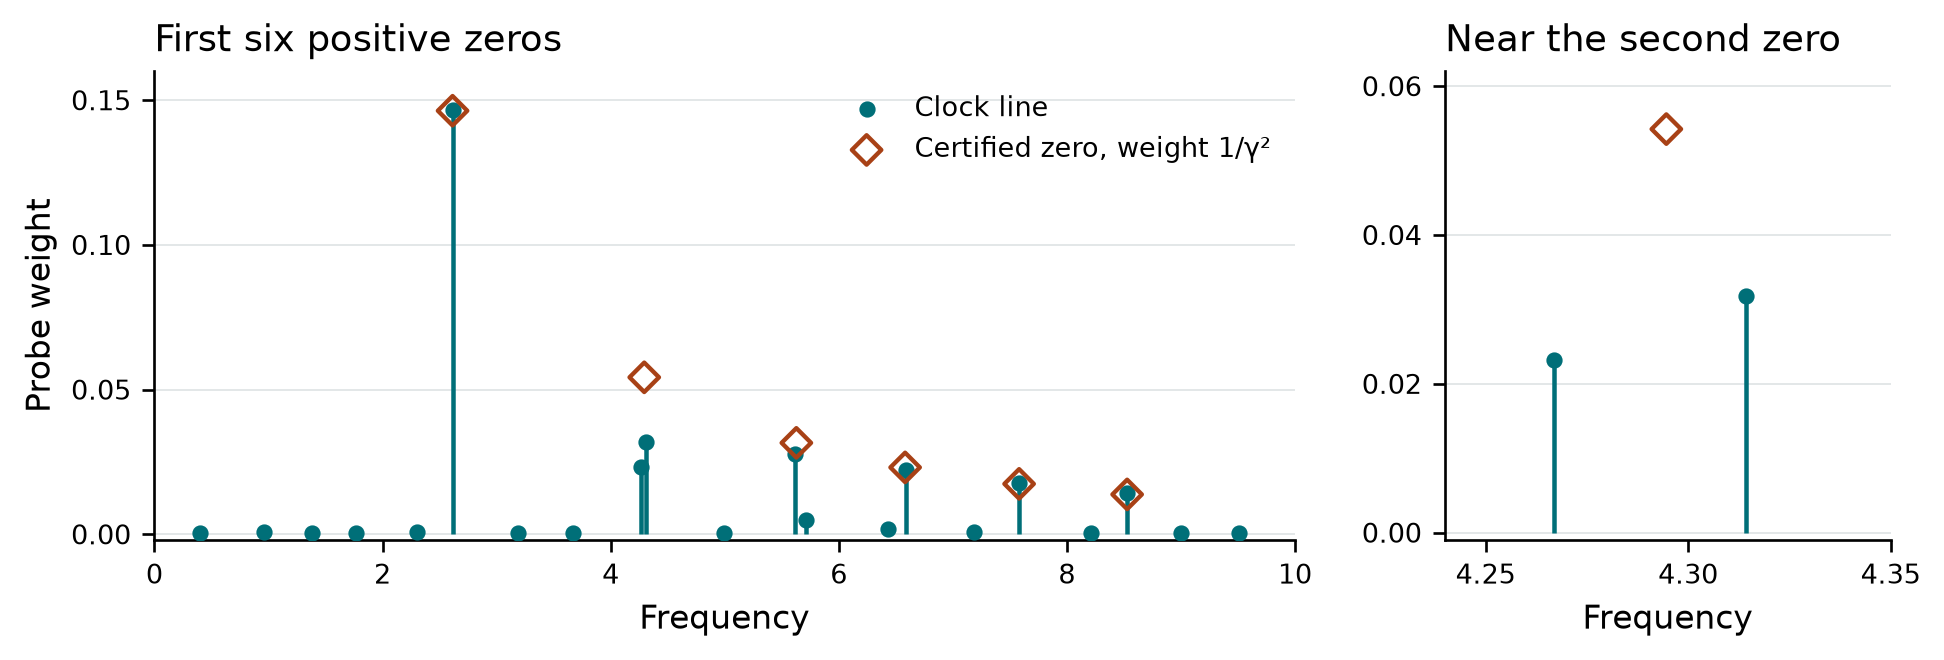
\includegraphics[width=.94\linewidth]{cubic-clock-spectrum.png}
\end{center}

\newpage
\section*{5. Which observable could survive a continuum limit?}
Before the first prime, $D''(L)=-2/L+O(1)$, so
$H(L)=4L\log(1/L)+O(L)$ as $L\downarrow0$.
For any unitary group $U(t)$ and Hilbert vector $v$,
$\|(I-U(L))\int_0^L U(u)v\,du\|^2\le4L^2\|v\|^2$.
Consequently a normalizable vector continuously injected at a constant
rate cannot reproduce the arithmetic, even with an unbounded Hamiltonian.

The second difference of an ordinary but sufficiently rough vector avoids
this obstruction. Under GRH set $U(L)e_\gamma=e^{i\gamma L}e_\gamma$ and
$w_\gamma=1/\gamma$ for every noncentral zero, repeating multiplicities.
Then $w\in\ell^2$ and $H(L)=\|(I-U(L))^2w\|^2$ exactly.
Conversely such a realization for all $L$ bounds $H$ by $16\|w\|^2$,
so the perfect-power theorem implies GRH. Every such realization requires
infinite mean absolute energy: the spectral theorem and
$|1-e^{ix}|^4\le16|x|$ would give
$H(L)\le16L\|\,|K|^{1/2}w\|^2$ for a state of finite mean absolute energy,
contradicting the logarithm at small $L$. For the displayed spectral
realization with generator $K$ the zero count of order $T\log T$ gives
$w\in\operatorname{Dom}|K|^s$ for $0\le s<1/2$, with divergence at $s=1/2$.
The nonzero slope jump $8\log(193)/\sqrt{193}$ at $L=\frac12\log193$
also rules out a bounded generator, whose second difference is real analytic.

\paragraph{The probe determines the visible frequencies.}
Suppose a clock realizes $H$ at all lengths. Write
$V_w(L)=\|(I-U(L))w\|^2$. This is bounded and $4V_w(L)-V_w(2L)=H(L)$,
so iteration gives
\[
 V_w(L)=\sum_{j\ge0}4^{-j-1}H(2^jL).
\]
GRH follows from boundedness of $H$. Since $A(1/2)>0$, the cubic $V$ is
then bounded too, and the same inversion shows $V_w=V$. If $\mu_w$ is the
spectral measure of $w$, the cosine transform of its even part is thus
determined up to a constant. Uniqueness of the Fourier transform of finite
measures gives
\[
 \left.\tfrac12(\mu_w+\mu_w^{-})\right|_{\mathbb R\setminus\{0\}}
   =\sum_{\gamma\ne0}\gamma^{-2}\delta_\gamma,
 \qquad \mu_w^{-}(E)=\mu_w(-E),
\]
where zeros are counted with multiplicity. Hence a successful global clock
would recover the absolute zero ordinates and their weights from its probe.
Mass at frequency zero and any spectrum orthogonal to the probe are invisible.

\paragraph{Reproduction.}
The certificate and spectrum can be reproduced together.
\begin{verbatim}
sage -python check_cubic_haar.py --figure cubic-clock-spectrum.png
\end{verbatim}
The finite tests use the prime-side formula and known local factors.
The asymptotic theorem uses real-axis nonvanishing and allows arbitrary
locations for the nonreal zeros within the critical strip.
Positivity at all perfect-power cutoffs remains open.

\begin{thebibliography}{9}
\bibitem{cubic} Project note, \emph{The cubic of discriminant 229},
section on the positive kernel and real-axis nonvanishing,
\texttt{cubic\_229.md}. The kernel is
$e^{v/2}\sum_{n\ge1}a_n K_0(2\pi n e^v/\sqrt{229})$ up to positive normalization.
\bibitem{suzuki} M. Suzuki, \href{https://arxiv.org/abs/2209.12832}
{\emph{Screw functions of Dirichlet series in the extended Selberg class}},
Int. J. Number Theory 21 (2025), 1815--1823.
\bibitem{form} M. Suzuki, \href{https://arxiv.org/abs/2606.09096}
{\emph{Weil's quadratic form via the screw function}} (2026).
\end{thebibliography}
\end{document}
